\subsection{Online Clustering}
\label{subsec:4c_online_clustering}

\subsubsection{Design}
\label{subsubsec:4c_design}

Detecting events in a stream of news articles will be achieved by using an online clustering approach.
An event is described by the occurrence of multiple news articles about the same story.
The events of interest for this application are the discovery of new stories and the extension of existing stories.
Thus we define our two types events as follows:

\begin{itemize}
    \item New event: A new cluster of news articles appears in the data stream, which describe the same story.
    \item Event extended: An existing story is extended by additional news articles.
\end{itemize}

HDBSCAN will be applied as the clustering method,
using the optimal settings discovered in the clustering method evaluation.
Additional preprocessing of news articles before clustering is going to be explored
as part of evaluation as well and will be implemented accordingly for the online clustering.

The clustering will be done batchwise over time, since HDBSCAN only supports static data sets.
Events are detected by comparing clusters from successive batches.
Figure \ref{fig:timeline} illustrates this with three batches,
where the resulting clusters from batch $t$ will be compared the previous result from batch $t - 1$,
while batch $t - 1$ was previously compared with batch $t - 2$.
In this example each batch only contains samples from a limited time period,
where $\triangle t$ stands for the time period between batches.
Since a batch does not contain the full set of samples, we have to consider the overlap between batches.
The size of the overlap is essential to find similar clusters different batches.
If a similar cluster already exists in the previous batch
the differences between these clusters are detected as a change in an existing event.
If no pair exists for a cluster from a current batch, this cluster will be regarded as a new event.
The similarity between clusters is based on the same assumptions
as for the scoring function described in Section \ref{subsubsec:4b_scoring_function}.

\begin{figure}[h]
    \centering

    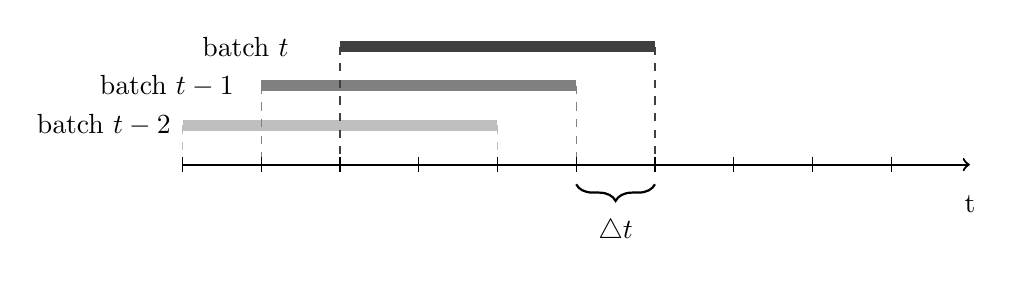
\begin{tikzpicture}[scale=1]

        \draw[lightgray, line width=4pt] (0,.5) -- (4,.5);
        \draw[lightgray, dashed] (0,.5) -- (0,0);
        \draw[lightgray, dashed] (4,.5) -- (4,0);
        \node[align=right] at (-1,.5) {batch $t - 2$};

        \draw[gray, line width=4pt] (1,1) -- (5,1);
        \draw[gray, dashed] (1,1) -- (1,0);
        \draw[gray, dashed] (5,1) -- (5,0);
        \node[align=right] at (-.2,1) {batch $t - 1$};

        \draw[darkgray, line width=4pt] (2,1.5) -- (6,1.5);
        \draw[darkgray, dashed] (2,1.5) -- (2,0);
        \draw[darkgray, dashed] (6,1.5) -- (6,0);
        \node[align=right] at (0.8,1.5) {batch $t$};

        \node[align=center] at (5.5,-0.85) {$\triangle t$};
        \node[align=center] at (10,-0.5) {t};

        \draw [thick,->] (0,0) -- (10,0);
        \foreach \x in {0,...,9} \draw (\x,0.1) -- (\x,-0.1);

        \draw [thick,decorate,decoration={brace,amplitude=6pt,raise=0pt,mirror}] (5,-0.25) -- (6,-0.25);

        \end{tikzpicture}

    \caption{Timeline showing the sliding window approach}
    \label{fig:timeline}
\end{figure}

The overlap between batches depends on the batch size and the number of new samples in $\triangle t$.
A high volume of incoming samples combined with a small batch sizes
would result in an overlap too small to find pairs of clusters will.
All clusters from the current batch will be detected as new in this case.
To decrease the negative impact on the event detection by peaks in the data stream,
we need a batch size which grows accordingly.
The ideal batch size therefore provides enough overlap between batches to find pairs of clusters
and small enough to allow for efficient processing.
We explore three different methods for determining the ideal batch size:

\begin{enumerate}
    \item \textbf{Fixed size}: The first method uses a fixed batch size, where each batch processes the most recent \textit{n} samples. This makes the clustering unstable against sudden peaks in the volume of incoming data, but we consider this method as useful benchmark for dynamic methods.
    \item \textbf{Size by hours}: This method uses a dynamic batch size by loading the samples from the last \textit{n} hours. This enables the batch size to increase and decrease with the volume of the data stream. The number of samples will be limited by an upper bound, to keep the space and time consumption of the clustering method reasonable. 
    \item \textbf{Size by incoming data}: This method defines the batch size relative to the incoming data. We count the number of new samples since the last batch and multiply it by a predefined factor. For example we want the new samples to be 1 \% of the overall clustering and therefore define the factor as 100. The batch size will be limited by a lower and an upper bound. The lower bound prevents the overlap between batches from getting too small. The upper bound is based on the same reasoning as mentioned in the previous method.
\end{enumerate}

The evaluation will use the MP-Score to measure the precision of the event detection,
since our model represents an event as a cluster.
True events can be extracted directly from the ground truth based on news articles from two successive batches.

\subsubsection{Implementation}
\label{subsubsec:4c_implementation}

The online clustering implemented for this thesis does not operate in a true online setting,
but rather it takes our existing test data and simulates a data stream over time.
The simulated approach allows us to directly compare the resulting events
with the ground truth and thus evaluate different settings.
The implementation is done with Python and runs in a similar dockerized environment as the evaluation framework.

\paragraph{Comparing clusters}
To detect events between batches of clusterings,
we have find pairs of clusters describing the same story.
This problem is solved in the evaluation framework as part of the scoring function,
by calculating the similarity for each possible cluster pair.
The resulting time complexity is $O(n^2)$, which we deemed acceptable for the static evaluation.
However in a dynamic setting such as the online clustering, performance is an important factor,
since it restricts the lengths of the time delta between batches and the overall batch size.
Thus we decided to use Locality-Sensitive Hashing (LSH)\cite{alex2015practical} to find similar clusters.
This reduces the time complexity to $O(log(n))$.
The implementation for LSH is provided by the datasketch library\cite{eric_zhu_2017_290602}.

% TODO explain LSH?

\paragraph{Detecting events}
Once we have found pairs of clusters, which represent the same story, detecting events becomes trivial.
For each pair we look for news articles, which are only present in the new cluster.
These articles are then summarized in as an extension of an existing event.
Clusters from the new batch without a matching cluster from the previous batch
are seen as new events.

\paragraph{Measuring the quality of events} 
Since events are themselves clusters of news articles,
we apply the MP-Score to measure detected events against events taken from the ground truth.
This gives an indication if the detected events contain the same news articles
as true events and thus the rate of false positives and false negatives.
Calculating the score is $O(n^2)$, but since the application runs on a simulated timeline,
time complexity is only a minor concern.

\paragraph{CLI}
The application provides a command line interface to run the simulation with different parameters
such as the start date, number of days to run and the batch size.

\begin{lstlisting}[caption=Command line interface for the online clustering, label={lst:cli_online_clustering}]
    usage: online_clustering.py [-h] [--full-cluster] [--verbose] [--rows ROWS]
                            [--full_rows FULL_ROWS] --date DATE
                            [--run_n_days RUN_N_DAYS] [--threshold THRESHOLD]

Run the batchwise clustering over a simulated stream of news articles.

required arguments:
  --date DATE           

optional arguments:
  -h, --help            show this help message and exit
  --full-cluster        run a full clustering once a day
                        default: False
  --verbose             
                        default: False
  --rows ROWS           number of samples to process per batch
                        default: 1000
  --full_rows FULL_ROWS
                        number of samples to process for the full clustering
  --run_n_days RUN_N_DAYS
                        number of days to run the batchwise clustering
                        default: 1
  --threshold THRESHOLD
                        similarity threshold for cluster matching
                        default: 0.75

\end{lstlisting}

% TODO clarify event vs topic vs story and be consistent with the usages!
